\section{The CMS experiment}
\label{sec:cms}
(describe the experiment in general, its discovery, mention the international collaboration) \\

\onehalfspacing Compact Muon Solenoid (CMS) is one of the major experiment at CERN's Large Hadron Collider (LHC) that have been built to search for new physics. CMS is designed to detect new particles produced in the LHC's high energy proton-proton and heavy-ion (Lead, Xenon) collisions. CMS will also measure the properties (mass, decay width, coupling) of already discovered particles like quarks and leptons with unprecedented precision and will be looking to discover completely new, beyond standard model of particle physics phenomena which will help us to get a better understanding of our Universe and may confirm or rule out multiverse hypothesis \cite{Chatrchyan:1129810}. This experiment has already confirmed the discovery of the most important particle in SM, the Higgs boson which gives mass to all bosons and fermions via electroweak symmetry breaking mechanism \cite{Chatrchyan:2012xdj}. It has also detected the decay of Higgs boson to a pair of photons, W bosons, bottom quarks and muons.  \\

The CMS experiment is one of the largest international scientific collaborations in history, involving 4300 particle physicists, engineers, technicians, students and support staff from 179 universities and institutes in 41 countries. \\

\subsection{CMS detector}
(describe the detector components and what they do) \\

The CMS detector is build around a large superconducting solenoid magnet and has a cylindrical shape with many concentric layers where various components of this detector are placed. It is placed at one of the collision points around the LHC ring and consists of Silicon tracker, Electromagnetic calorimeter, Hadron calorimeter and Muon chambers as shown in the left part of Fig. 4. \\

The large solenoid magnet bend charged particles and studying the path taken by these charged particles produced in proton-proton collisions using Silicon pixel detector (innermost part of CMS tracker) as they fly away from the interaction point, we can identify the charge of a particle as positive and negative charged particle tracks bend in opposite directions by the magnetic field and can also be used to calculate the momentum of the charged particle using curvature of the track as shown in the right part of Fig. 4. \\

Energies of various particles produced in the collision is measured by calorimeters. The Electromagnetic Calorimeter measures the energy of electrons and photons while the Hadron Calorimeter measures energy of hadrons which are particle made up of quarks and gluons. \\

The Muon chambers are used to detect muons that are charged particles just like electrons but 206 times heavier. Muons can travel several metres without interacting thats why muon chambers are placed at the periphery of the CMS experiment. Muons are important particles to detect because they are produced in the decay of new particles and are helpful in exploring physics beyond SM.



\begin{figure}[H]
  \centering
  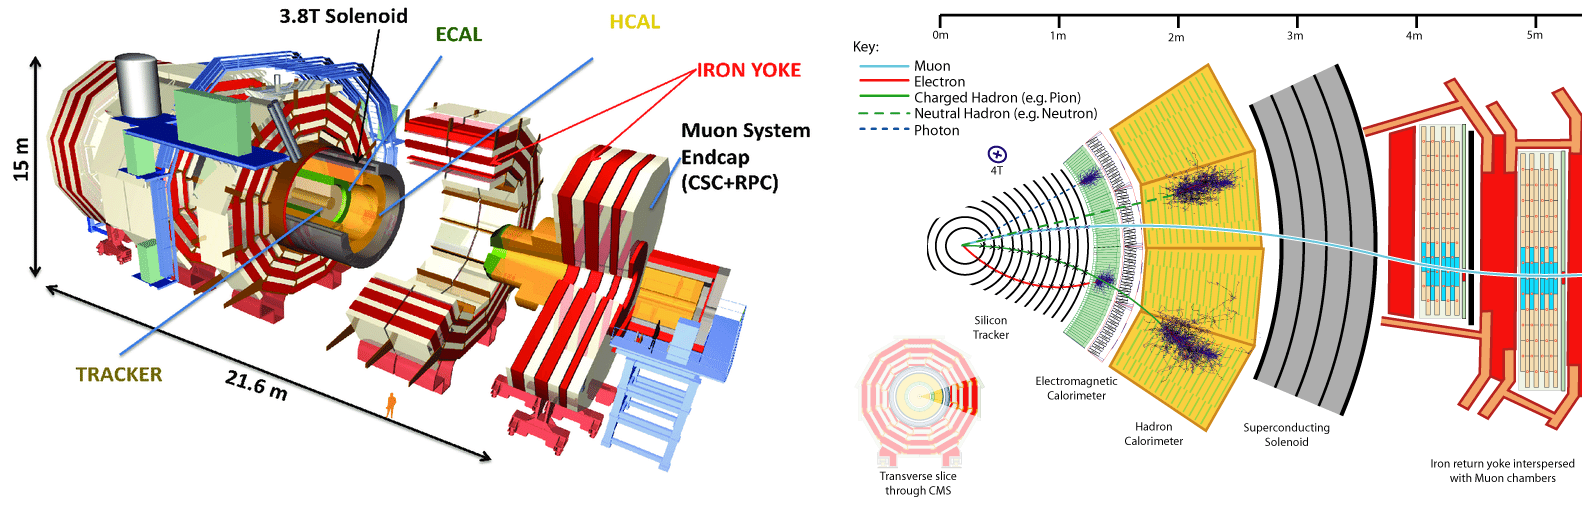
\includegraphics[width=1\columnwidth]{./cmsdetector_merged.png}
  \caption{Left: 3D design of CMS detector showing various concentric layers. Right: \onehalfspacing Transverse view of the CMS detector showing the silicon tracker, electromagnetic calorimeter, hadron calorimete##r, superconducting solenoid and muon chambers. \cite{Chatrchyan:2008aa}}
  \label{fig:CMSdetector}
\end{figure}





\subsection{The Pixel detector}

The pixel detector is the innermost of CMS tracker that contains 60 million pixels and these pixels assist in tracking the paths of particles emerging from the collision point. It is the nearest detector to the beam pipe and so will be vital in reconstructing the tracks of very short-lived particles. As it is very close to the collision point which means that the number of particles passing through is huge, the rate of particles received at 8cm from the beam line will be around 10 million particles per square centimetre per second. This feature is used to calculate the instantaneous luminosity $(L_{inst})$ by counting the number of pixel clusters which are collection of pixels hit by a track. The pixel detector is able to disentangle and reconstruct all the tracks left by the particles coming from the interaction point and has a long duration of 10 years. \\

The CMS Run 2 pixel detector consists of four concentric barrel layers (L1-L4) at radii of 29, 68, 109 and 160 mm and three disks (D1-D3) on each end at distances of 291, 396, and 516 mm from the center of the detector. It is built from 1856 segmented silicon sensor modules, where 1184 modules are used in the barrel pixel detector (BPIX) and 672 modules are used for the forward disks (FPIX) \cite{TrackerGroupoftheCMS:2020bgg}. \\

Each layer of the pixel detector is spilt into tiny square segments with each segment containing a silicon sensor having dimensions 100$\mu$m $\times$ 150$\mu$m as shown in the right part of Fig. 5. When a charged particle passes through this silicon sensor, it transfers energy to silicon atoms which causes electrons to be ejected from it creating electron-hole pairs. Each pixel uses an electric current to collect these charges on the pixel surface as a small electric signal. A electronic silicon chip is attached to each segment which amplifies the signal. The particle trajectory is deduced by knowing the hit pixels and as the pixel detector is made of two dimensional segments with four layers, we can create a three-dimensional picture of the path taken by the charged particle.



\begin{figure}[H]
  \centering
  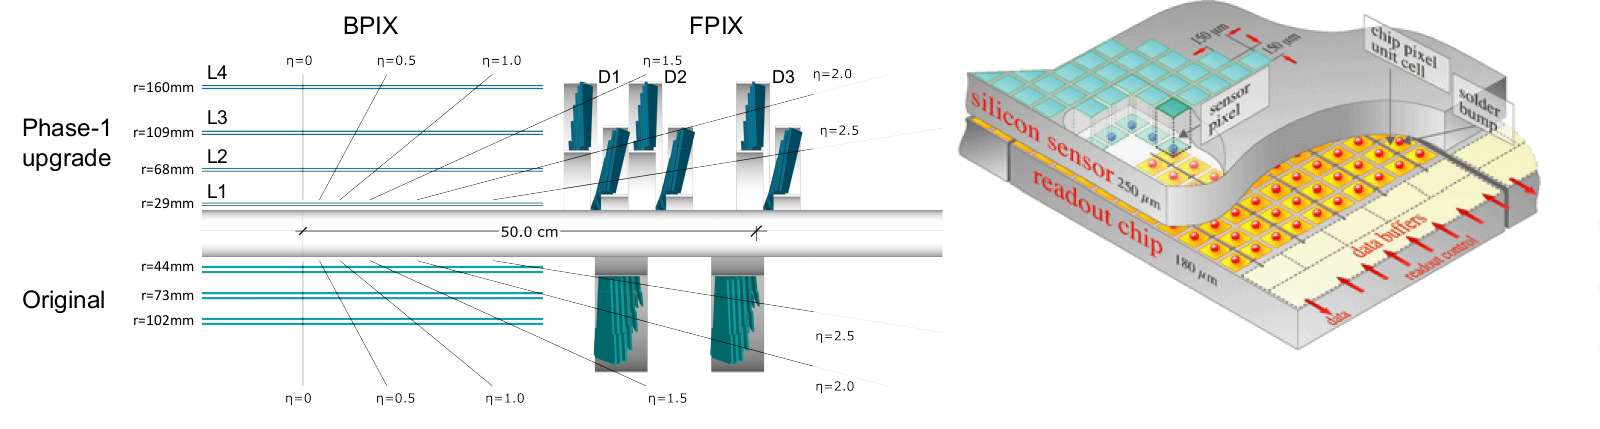
\includegraphics[width=1 \columnwidth]{./pixeldetector_merged1.png}
  \caption{Left: Layout of the CMS Run 2 pixel detector compared to the original detector layout, in longitudinal view. Right: pixel detector diagram showing size of Silicon sensor, readout chip and data buffers.}
  \label{fig:LHC}
\end{figure}


